\section{Introduction}

With the development of computing technology, data storage continues to grow to high values. The development of data usage and storage is\begin{figure}[ht]
    \centering
    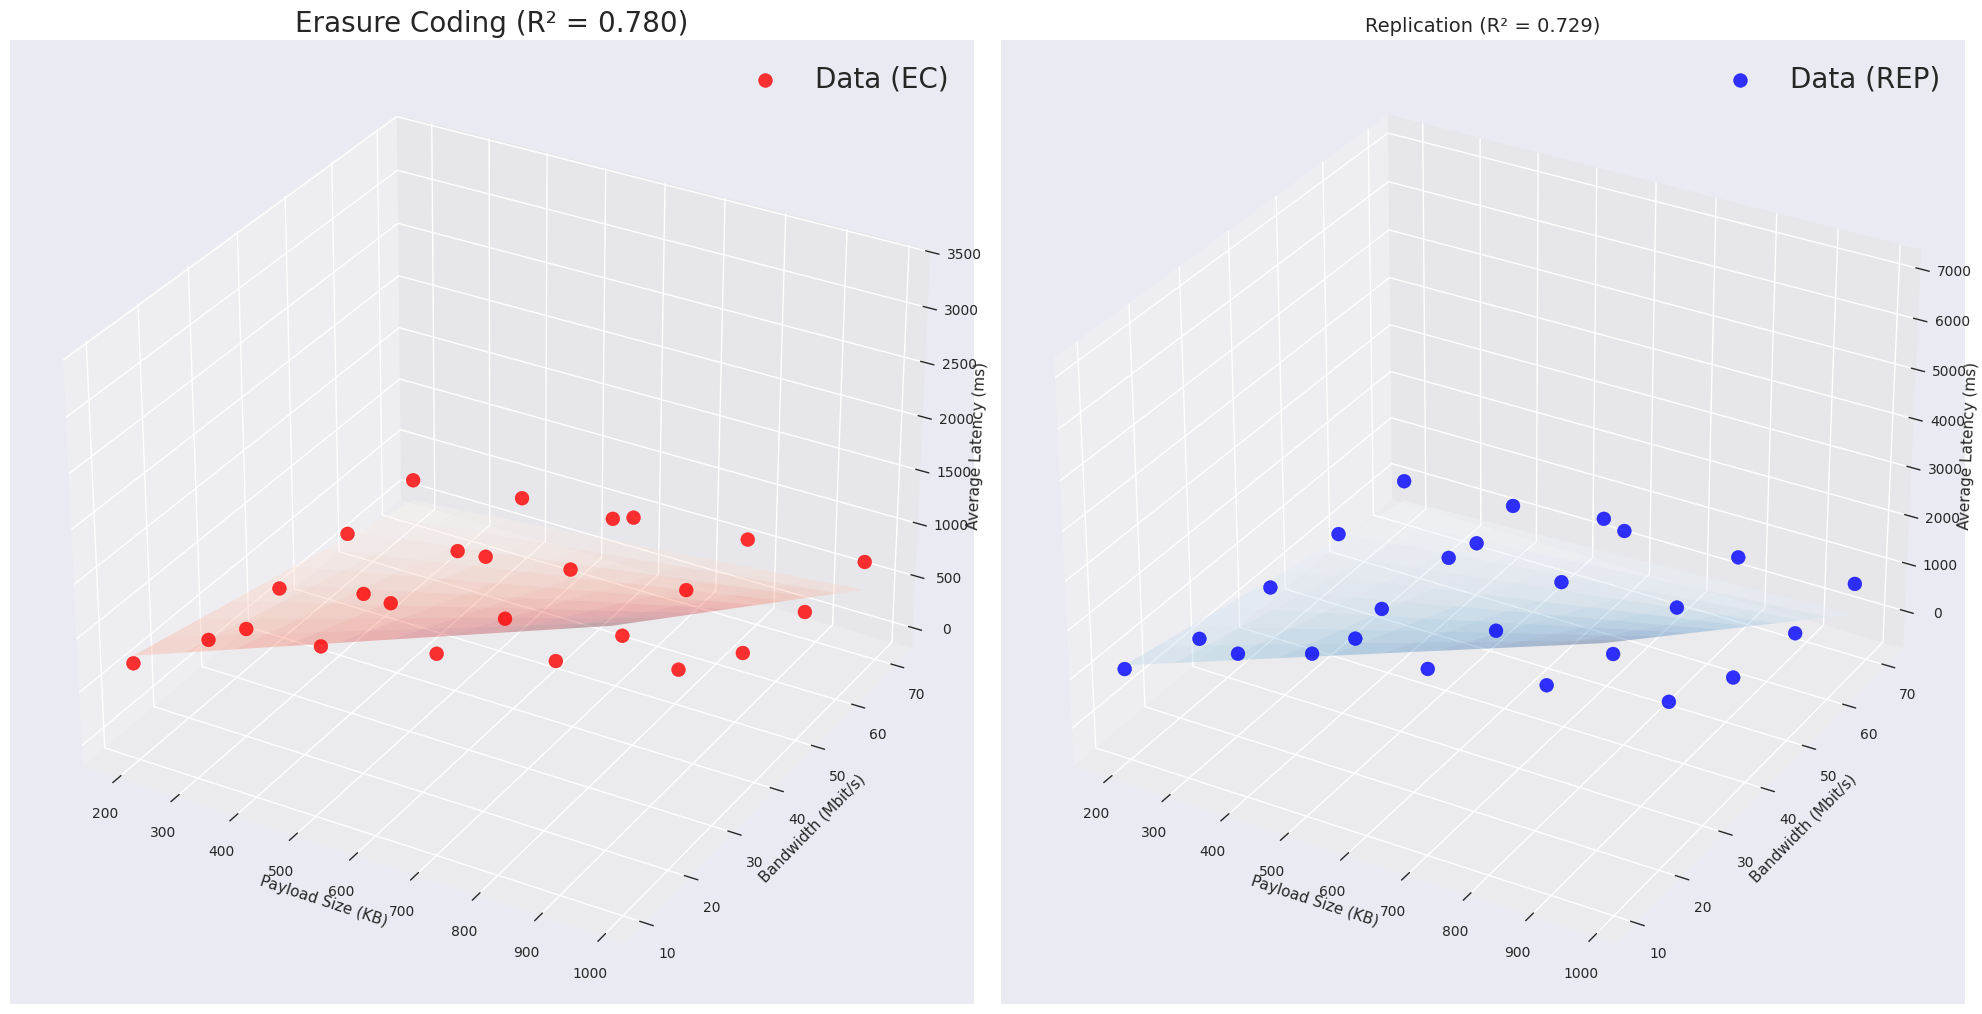
\includegraphics[width=\columnwidth]{resources/chapter-4/write_bigload_avgnet_regression.png}
    \caption{Three-Dimensional Performance Model for Write Operations}
    \label{fig:write-regression-model}
\end{figure}n by the emergence of cloud computing technology, data needs for artificial intelligence training based on machine learning, and general improvement in data quality in files.

Along with this, the use of systems has become increasingly intensive. This intensive use creates a need for high resilience so that these systems can continue to operate, especially in facing the possibility of component failure and data loss \cite{weatherspoon2002erasure}. In this case, data redundancy solutions become very important. Traditionally, replication techniques are used to duplicate data to multiple nodes. However, with the growing need for data in operations, this approach consumes increasingly large storage capacity and significantly increases operational costs.

Another solution to address these failures is erasure coding. With the application of erasure coding, data storage requirements can be reduced while maintaining data integrity and resilience, especially in distributed system environments using multiple devices simultaneously \cite{balaji2018erasure}. However, erasure coding requires higher computational resources compared to replication in its implementation. This causes high latency and response time from the services created. In fact, many application services make low latency a requirement in their operations \cite{dean2013tail}.

The fundamental trade-off can be expressed mathematically. For write operations, the total response time for erasure coding ($T_{EC}$) versus replication ($T_{REP}$) can be modeled as:

\begin{equation}
T_{EC} = T_{encoding} + T_{network\_reduced} + T_{consensus}
\end{equation}

\begin{equation}
T_{REP} = T_{network\_full} + T_{consensus}
\end{equation}

Where $T_{network\_reduced} < T_{network\_full}$ due to the smaller total data volume transmitted in erasure coding, but $T_{encoding} > 0$ represents the computational overhead. The performance crossover occurs when $T_{EC} < T_{REP}$.

However, besides adding computation, the application of erasure coding in a system reduces the overall data size to provide data integrity and resilience. Reducing data size can also cause a decrease in the size of data sent to other nodes. Thus, erasure coding has the potential to have conditions when the data size is large enough and the network is slow enough that the response time is lower in certain operations compared to performing the same operations on a replication system.

\section{Related Work}

Several studies have explored the application of erasure coding in distributed storage systems. Weatherspoon and Kubiatowicz \cite{weatherspoon2002erasure} demonstrated the effectiveness of erasure codes in providing fault tolerance with lower storage overhead compared to replication. Balaji et al. \cite{balaji2018erasure} analyzed the trade-offs between storage efficiency and computational overhead in erasure-coded systems.

Recent work has focused on optimizing erasure coding for specific workloads and system architectures. However, limited research has specifically addressed the performance characteristics of erasure coding in distributed key-value store databases, particularly regarding response time thresholds where erasure coding outperforms replication.

\section{System Design and Implementation}

\subsection{Architecture Overview}

The implemented distributed key-value store system employs a modular architecture designed to support both erasure coding and replication mechanisms under identical conditions. The system consists of several key components:

\begin{itemize}
\item \textbf{Node}: Basic computational unit managing data storage, retrieval, and consensus operations
\item \textbf{Data Collector}: External benchmarking system for systematic performance data collection
\item \textbf{Benchmark Component}: Automated testing framework with configurable parameter variations
\item \textbf{In-memory Key-Value Store}: High-performance cache layer to optimize read operations
\item \textbf{Persistent Database}: RocksDB-based storage layer for durability
\item \textbf{Consensus Layer}: OmniPaxos protocol ensuring data consistency across distributed nodes
\end{itemize}

\subsection{Erasure Coding Implementation}

The erasure coding implementation utilizes Reed-Solomon algorithms with configurable data and parity shard ratios. The encoding process transforms original data into multiple fragments, where any subset of fragments can reconstruct the original data. This approach provides fault tolerance equivalent to replication while requiring significantly less storage space.

The system implements static erasure coding configuration with:
\begin{itemize}
\item Reed-Solomon encoding with systematic codes
\item Configurable data-to-parity shard ratios
\item Parallel encoding/decoding operations
\item Fragment distribution across multiple nodes
\end{itemize}

\subsection{Consensus and Consistency}

The OmniPaxos consensus protocol ensures strong consistency across all nodes regardless of the storage mechanism used. This protocol choice enables fair performance comparison between erasure coding and replication by maintaining identical consistency guarantees.

\subsection{Performance Monitoring and Tracing}

The system incorporates comprehensive performance monitoring capabilities:
\begin{itemize}
\item Operation-level latency tracing
\item Network bandwidth utilization monitoring  
\item CPU usage tracking during encoding/decoding
\item Memory allocation and garbage collection profiling
\item Disk I/O performance analysis
\end{itemize}

These monitoring capabilities enable detailed analysis of performance bottlenecks and validation of theoretical predictions.

\section{Experimental Setup and Methodology}

\subsection{Controlled Test Environment}

The experiments are conducted in a carefully controlled virtual machine environment with advanced traffic control capabilities for precise network simulation. This setup enables systematic variation of network parameters while maintaining reproducible conditions across multiple test runs.

The experimental infrastructure includes:
\begin{itemize}
\item Virtualized compute nodes with controlled resource allocation
\item Software-defined network simulation with configurable bandwidth and latency
\item Automated benchmarking framework for systematic parameter sweeping
\item Comprehensive performance monitoring and data collection systems
\end{itemize}

\subsection{Multi-Scenario Testing Framework}

The benchmark system implements three distinct testing scenarios designed to explore different operational environments:

\textbf{Scenario 1 - High Performance Environment}: Simulates modern data center conditions with high bandwidth (10 Gbps) and small payloads (1KB), designed to favor replication performance.

\textbf{Scenario 2 - Resource Constrained Environment}: Models edge computing or IoT scenarios with limited bandwidth (1 Mbps) and large payloads (200-1000KB), designed to potentially favor erasure coding.

\textbf{Scenario 3 - Realistic Network Conditions}: Represents typical internet connectivity with moderate bandwidth (10-70 Mbps) and variable payload sizes, designed to identify performance crossover points.

\subsection{Parameter Space Exploration}

The experimental design systematically varies two critical parameters:
\begin{itemize}
\item \textbf{Network Bandwidth}: 1Mbps, 10-70Mbps (incremental), and 10Gbps
\item \textbf{Payload Size}: 1KB, 200KB, 400KB, 600KB, 800KB, and 1000KB
\end{itemize}

This parameter matrix generates 25 distinct experimental conditions, enabling comprehensive analysis of the performance landscape and mathematical modeling of system behavior.

\subsection{Advanced Performance Metrics}

Beyond basic response time measurements, the system collects comprehensive performance data:

\textbf{Latency Components}:
\begin{itemize}
\item Network transmission time
\item Encoding/decoding computational overhead
\item Consensus protocol latency
\item Storage I/O operations time
\item Memory allocation and management overhead
\end{itemize}

\textbf{System Resource Utilization}:
\begin{itemize}
\item CPU utilization during encoding operations
\item Memory consumption patterns
\item Network bandwidth utilization efficiency
\item Storage space requirements and efficiency
\end{itemize}

\subsection{Statistical Analysis Framework}

The experimental methodology incorporates rigorous statistical analysis:
\begin{itemize}
\item Multiple trial runs for statistical significance
\item Ridge regression modeling to handle noise and prevent overfitting
\item Three-dimensional performance surface modeling
\item Boundary condition analysis for performance crossover identification
\item Confidence interval calculation for performance predictions
\end{itemize}

This comprehensive methodology ensures robust and reproducible results while enabling mathematical modeling of system performance characteristics.

\section{Results and Analysis}

\subsection{Write Operation Performance}

The experimental results demonstrate that erasure coding exhibits a threshold condition where response time becomes lower than replication for write operations. Through comprehensive benchmarking across three distinct scenarios, we identify specific conditions where this performance crossover occurs.

\subsubsection{Extreme Scenarios Analysis}

Figure \ref{fig:write-performance-comparison} illustrates the performance characteristics under two extreme conditions. In high-bandwidth environments (10 Gbps) with small payloads (1KB), replication consistently outperforms erasure coding due to the computational overhead of encoding operations. However, in constrained bandwidth environments (1 Mbps) with large payloads (200-1000KB), erasure coding demonstrates superior performance by reducing the total data transmission requirements.

\begin{figure}[ht]
    \centering
    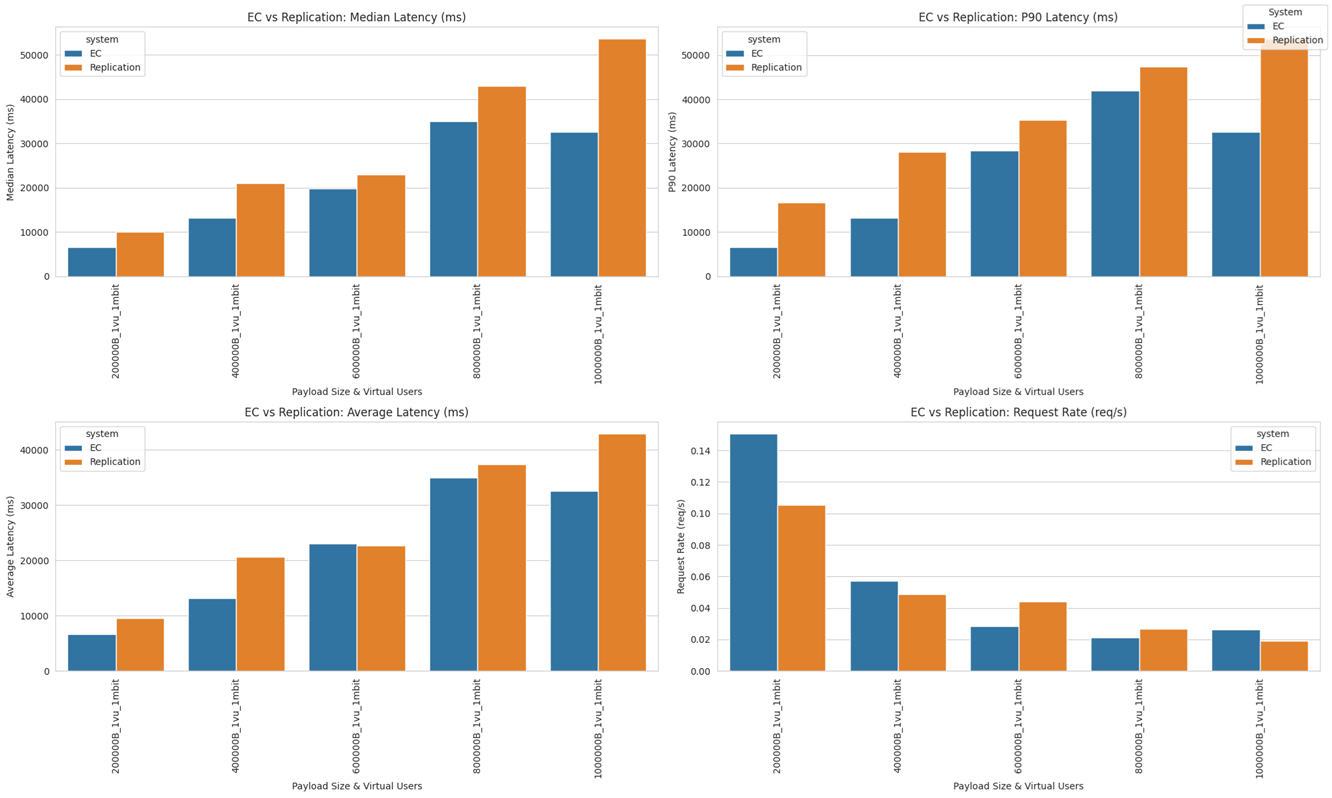
\includegraphics[width=\columnwidth]{resources/chapter-4/write_bigload_slownet.png}
    \caption{Write Performance on Low Bandwidth with Large Payload}
    \label{fig:write-performance-comparison}
\end{figure}

\subsubsection{Mathematical Performance Modeling}

To precisely determine the performance crossover points, we conducted regression analysis using ridge regression to model the relationship between bandwidth, payload size, and response time. The resulting three-dimensional performance model reveals the boundary conditions where erasure coding outperforms replication.

\begin{figure}[ht]
    \centering
    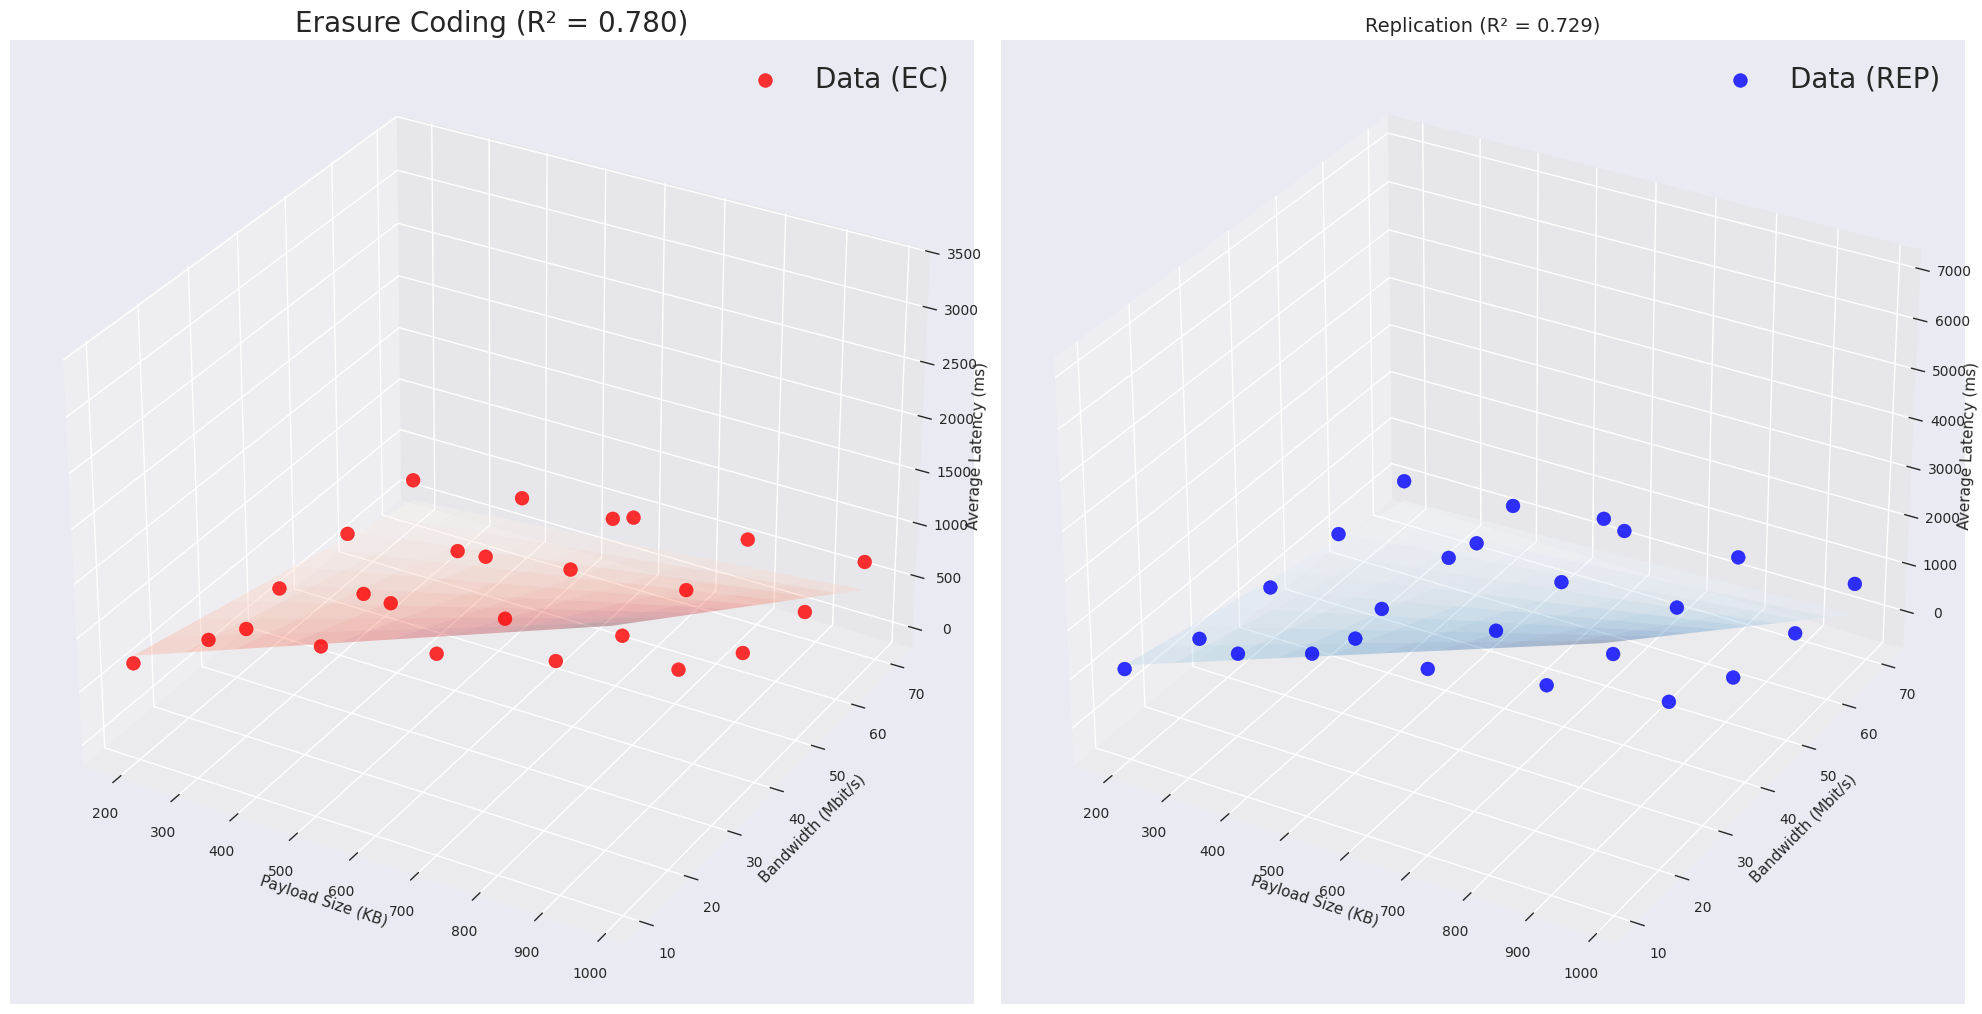
\includegraphics[width=\columnwidth]{resources/chapter-4/write_bigload_avgnet_regression.png}
    \caption{Three-Dimensional Performance Model for Write Operations}
    \label{fig:write-regression-model}
\end{figure}

\subsubsection{Performance Boundary Analysis}

Figure \ref{fig:performance-boundary} presents the derived performance boundary curve, which mathematically defines the threshold conditions. Points above the curve indicate scenarios where erasure coding outperforms replication, while points below favor replication. This boundary demonstrates that erasure coding becomes advantageous when:
\begin{itemize}
\item Network bandwidth is limited ($\leq$10Mbps for payloads $\geq$500KB)
\item Payload size is sufficiently large relative to available bandwidth
\item The ratio of encoding overhead to transmission time reduction favors erasure coding
\end{itemize}

\begin{figure}[ht]
    \centering
    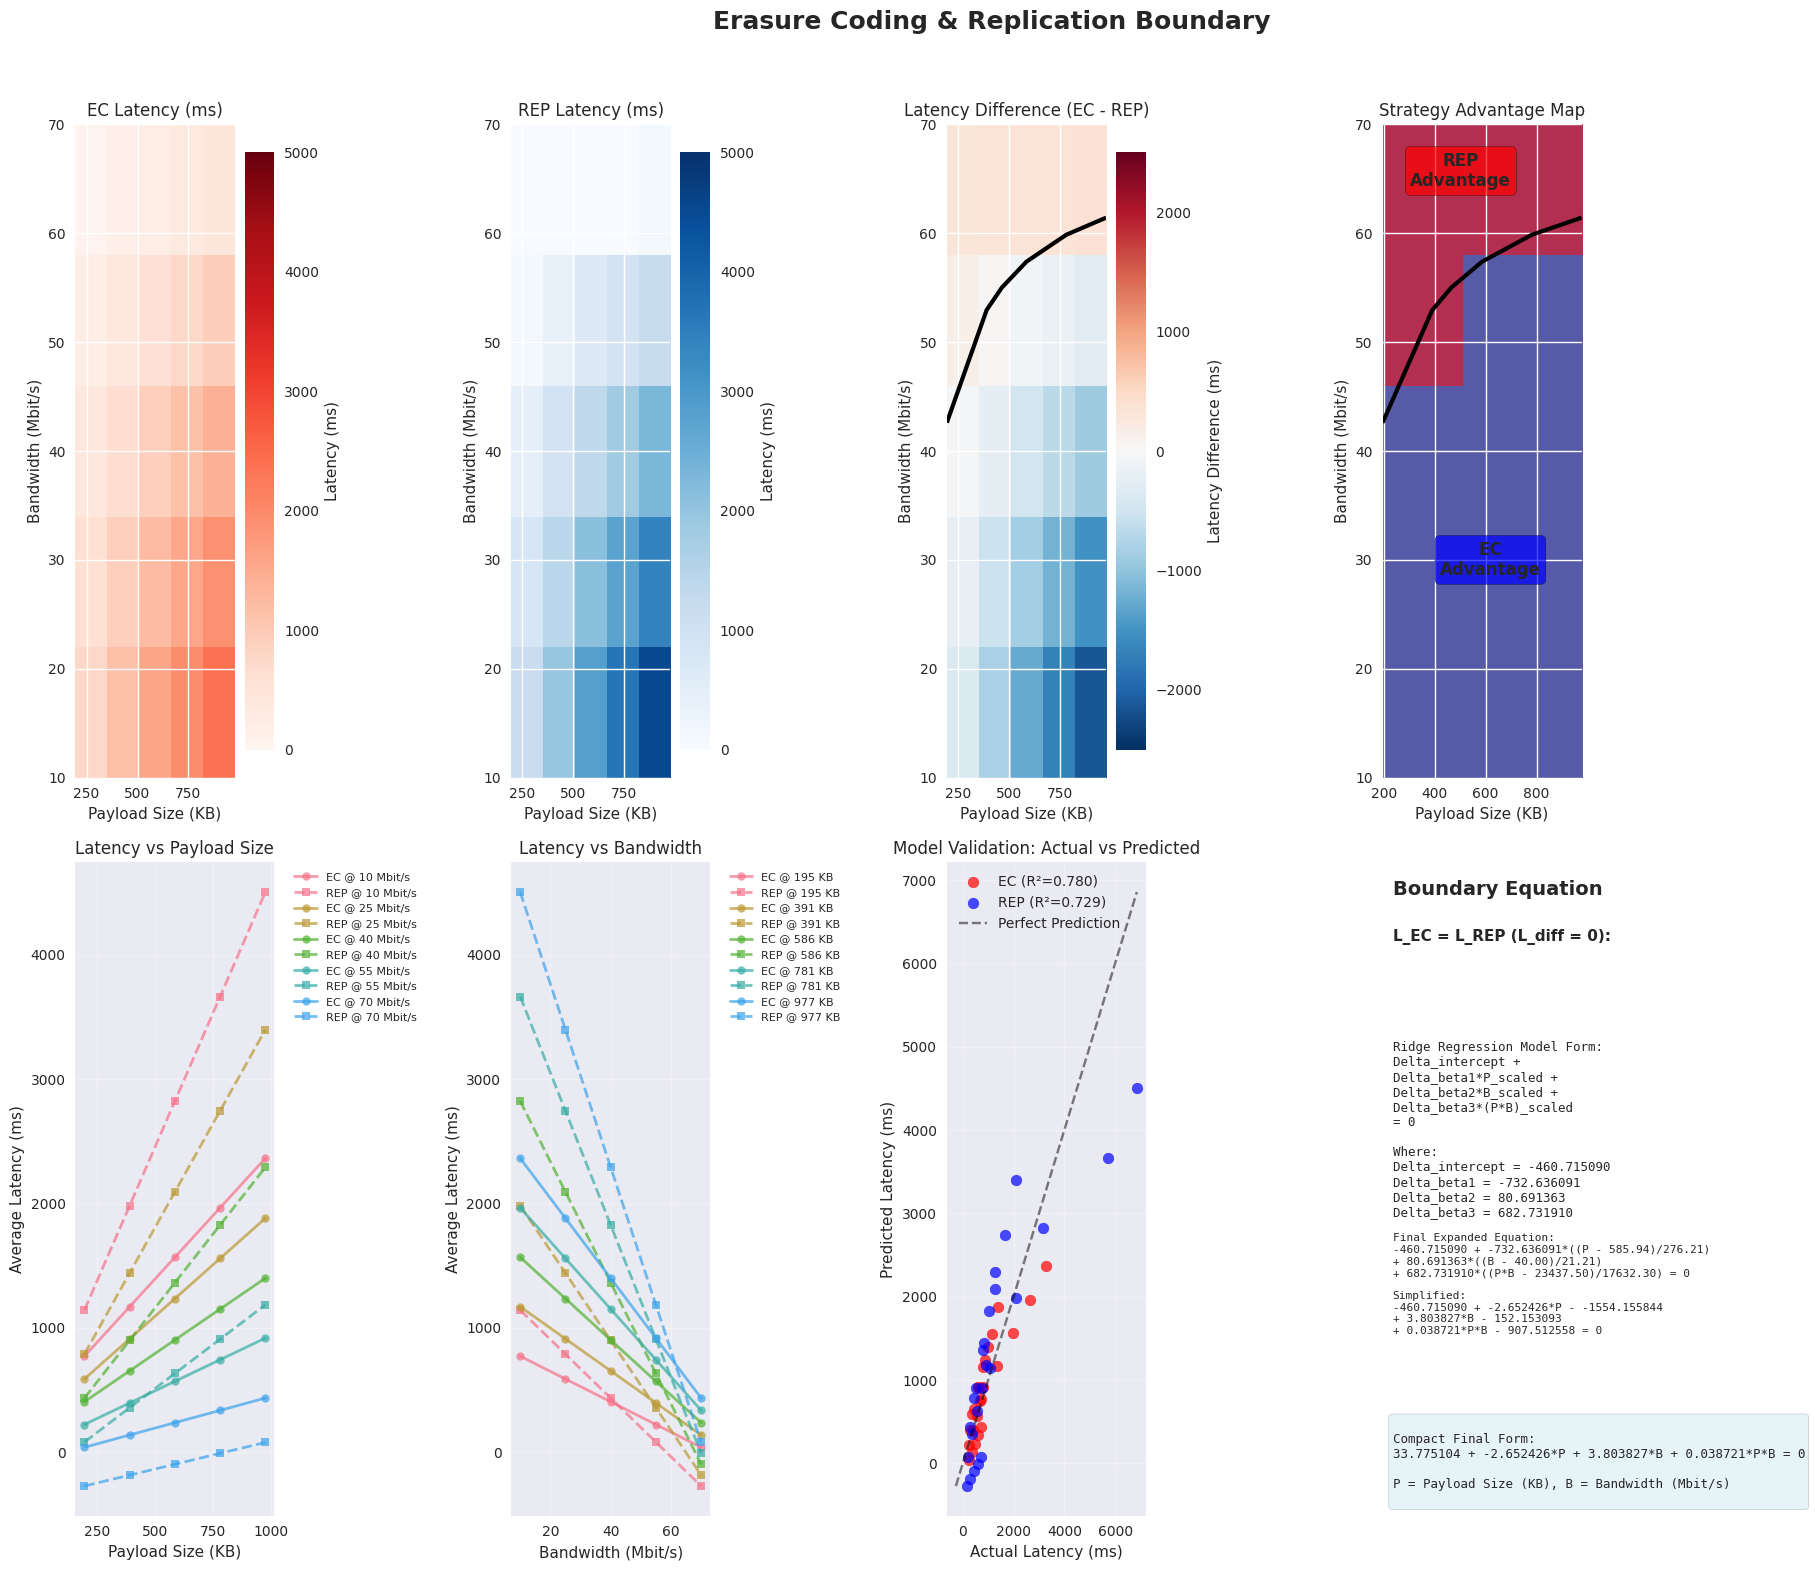
\includegraphics[width=\columnwidth]{resources/chapter-4/write_bigload_avgnet_boundary.png}
    \caption{Performance Boundary Analysis Between Erasure Coding and Replication}
    \label{fig:performance-boundary}
\end{figure}

\subsubsection{Performance Heatmap Visualization}

The comprehensive performance analysis across varying bandwidth and payload combinations is visualized in Figure \ref{fig:write-heatmap}. Blue regions indicate erasure coding superiority, while red regions show replication advantages. This visualization clearly demonstrates the parameter space where each approach excels.

\begin{figure}[ht]
    \centering
    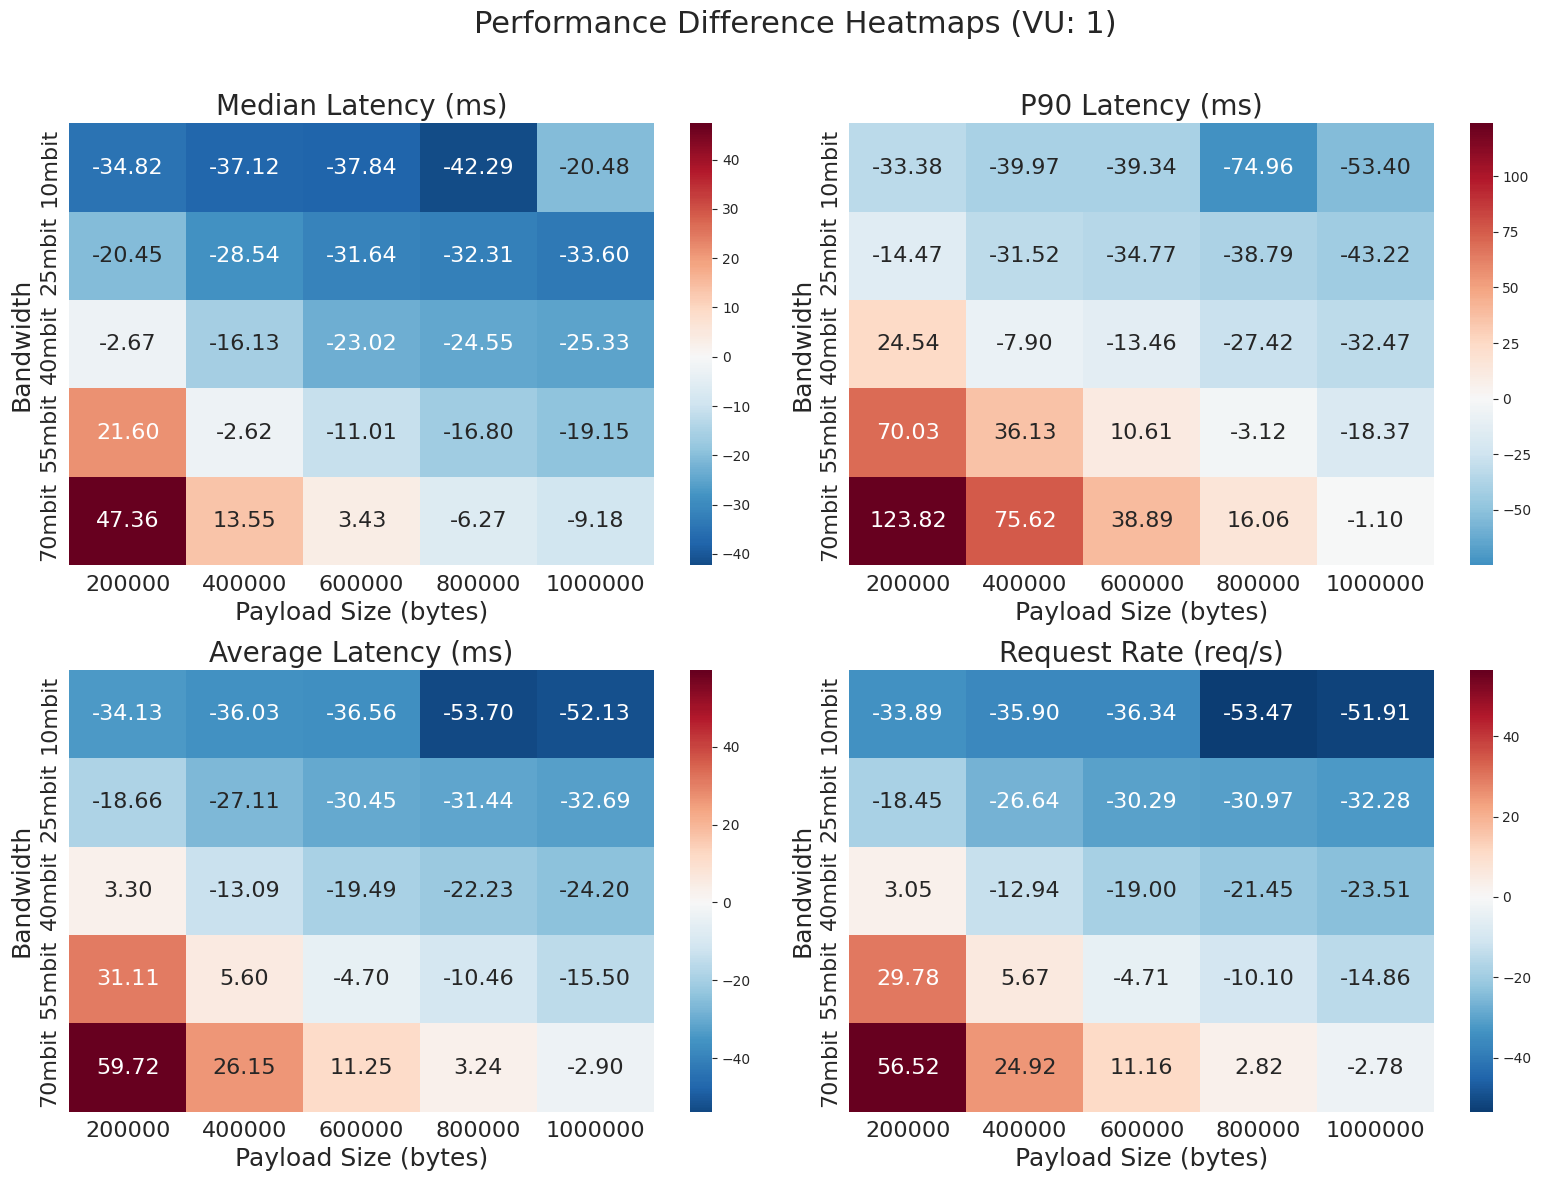
\includegraphics[width=\columnwidth]{resources/chapter-4/write_bigload_avgnet_heatmap.png}
    \caption{Performance Heatmap: Erasure Coding vs Replication for Write Operations}
    \label{fig:write-heatmap}
\end{figure}

\subsection{Read Operation Performance}

For read operations, replication consistently outperforms erasure coding across all tested parameter combinations. This performance difference is mathematically proven through latency analysis.

\subsubsection{Mathematical Latency Analysis}

The latency for erasure coded reads can be expressed as:
\begin{equation}
L_{EC} = T_{data} + T_{reconstruction} + T_{shard}
\label{eq:ec-read-latency}
\end{equation}

While replication read latency is simply:
\begin{equation}
L_{REP} = T_{data}
\label{eq:rep-read-latency}
\end{equation}

The performance difference is therefore:
\begin{equation}
\Delta L = L_{EC} - L_{REP} = T_{reconstruction} + T_{shard}
\label{eq:read-latency-diff}
\end{equation}

This fundamental difference ensures that replication will always outperform erasure coding for read operations, as reconstruction and shard retrieval operations add unavoidable overhead.

\begin{figure}[ht]
    \centering
    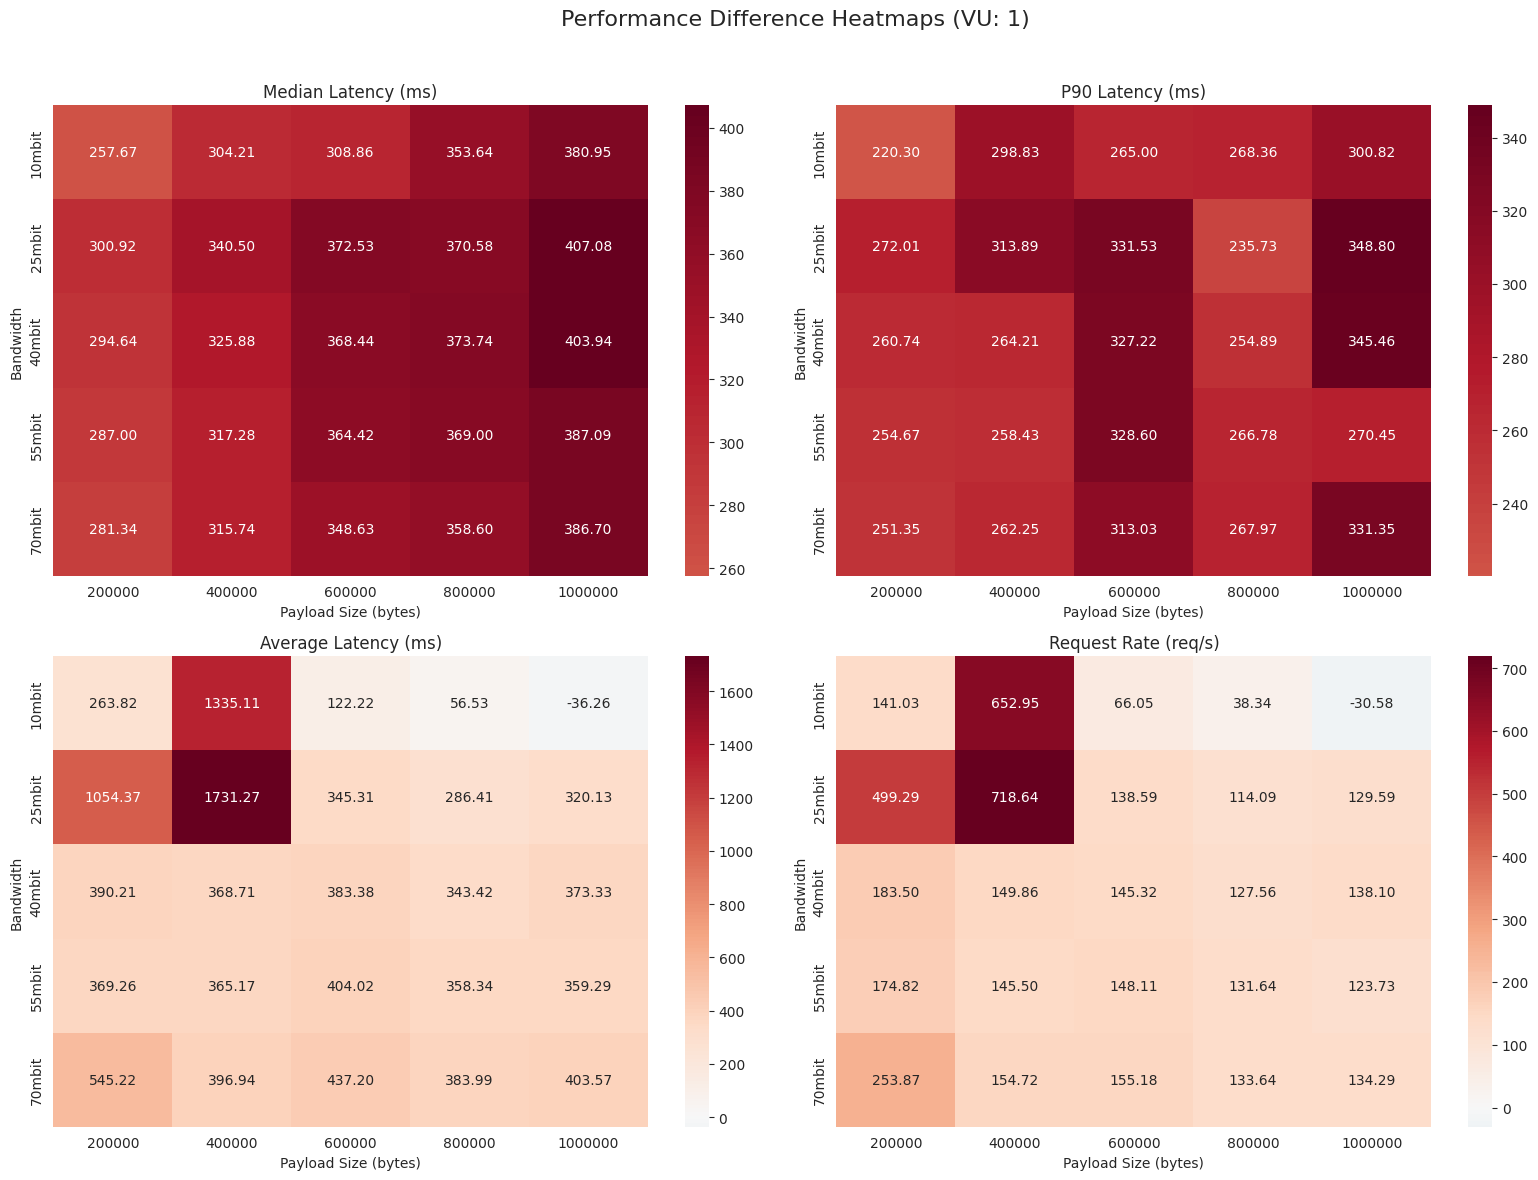
\includegraphics[width=\columnwidth]{resources/chapter-4/read_bigload_avgnet_heatmap.png}
    \caption{Read Performance Heatmap Showing Consistent Replication Advantage}
    \label{fig:read-heatmap}
\end{figure}

\subsubsection{Impact of In-Memory Caching}

The implementation includes an in-memory store that can mitigate read performance penalties. With caching, the effective erasure coding read latency becomes:
\begin{equation}
L_{EC} = T_{data} + (T_{reconstruction} + T_{shard}) \times (1 - \text{hit rate})
\label{eq:ec-read-latency-cached}
\end{equation}

This demonstrates that high cache hit rates can significantly reduce the performance gap, though replication maintains its fundamental advantage.

\subsection{Storage Efficiency}

Erasure coding demonstrates significant advantages in storage efficiency, requiring approximately 50\% less storage space compared to triple replication while maintaining equivalent fault tolerance capabilities. This storage efficiency becomes particularly valuable in large-scale deployments where storage costs are significant.

\section{Discussion}

\subsection{Theoretical Framework and Practical Implications}

The research establishes a theoretical framework for understanding the performance trade-offs between erasure coding and replication in distributed key-value stores. The mathematical modeling reveals that the performance crossover is fundamentally governed by the relationship between computational overhead and network transmission efficiency.

The derived performance boundary curve provides practical guidance for system architects. Erasure coding is most suitable for distributed key-value store databases operating under specific conditions:
\begin{itemize}
\item Large data objects (>500KB) where encoding overhead is amortized
\item Limited network bandwidth environments (<10Mbps)
\item Write-heavy workloads where storage efficiency is critical
\item Geographically distributed systems with high inter-node latency
\item Cost-sensitive deployments prioritizing storage optimization
\end{itemize}

\subsection{System Design Considerations}

The analysis reveals several critical design considerations:

\textbf{Adaptive System Architecture}: The clear delineation of performance boundaries suggests that adaptive systems could dynamically switch between erasure coding and replication based on real-time workload characteristics, data size patterns, and network conditions.

\textbf{Caching Strategy}: The mathematical analysis of in-memory caching demonstrates that strategic caching can significantly mitigate read performance penalties in erasure coded systems. Systems with predictable access patterns could leverage high cache hit rates to approach replication performance for reads while maintaining erasure coding benefits for writes.

\textbf{Workload Characterization}: The fundamental performance differences between read and write operations suggest that workload characterization is crucial for system optimization. Write-heavy workloads with large objects benefit most from erasure coding, while read-heavy workloads favor replication.

\subsection{Broader Implications for Distributed Systems}

The findings have broader implications beyond key-value stores:

\textbf{Edge Computing}: In edge computing scenarios with limited bandwidth to central data centers, erasure coding provides both performance and storage benefits for large data synchronization tasks.

\textbf{IoT Data Management}: Internet of Things applications generating large sensor data payloads can benefit from erasure coding when transmitting over constrained networks.

\textbf{Backup and Archival Systems}: Long-term storage systems handling large files benefit significantly from erasure coding's storage efficiency while tolerating higher read latencies.

\subsection{Limitations and Model Validity}

The current implementation and analysis have several important limitations:

\textbf{Static Configuration}: The erasure coding implementation uses fixed parameters (data and parity shards), limiting adaptability to varying workload characteristics.

\textbf{Environmental Constraints}: The regression model is valid only under the specific experimental conditions and hardware configurations tested. Different computational capabilities, memory speeds, or network characteristics would require model recalibration.

\textbf{Simplified Workload}: The analysis focuses solely on read and write operations without considering complex transaction patterns, consistency requirements, or failure scenarios that occur in production systems.

\textbf{Network Simulation}: Testing was conducted in controlled virtual environments with simulated network conditions, which may not fully capture the complexity and variability of real-world network behavior.

\section{Conclusion}

This research provides a comprehensive performance analysis of erasure coding versus replication in distributed key-value store databases, establishing both theoretical foundations and practical guidelines for system design decisions.

\subsection{Key Contributions}

The study makes several significant contributions to the field:

\textbf{Mathematical Performance Modeling}: We developed a rigorous mathematical framework using regression analysis that precisely defines the performance boundary between erasure coding and replication. This model enables system architects to predict performance characteristics based on bandwidth and payload size parameters.

\textbf{Quantitative Performance Boundaries}: The research establishes that erasure coding outperforms replication for write operations when network bandwidth is limited ($\leq$10Mbps) and payload sizes are large ($\geq$500KB). These thresholds provide concrete guidance for technology selection.

\textbf{Fundamental Read Operation Analysis}: Through mathematical proof, we demonstrate that replication will always outperform erasure coding for read operations due to the unavoidable overhead of data reconstruction and shard retrieval, quantified as $\Delta L = T_{reconstruction} + T_{shard}$.

\textbf{Storage Efficiency Quantification}: Erasure coding achieves approximately 50\% storage reduction compared to triple replication while maintaining equivalent fault tolerance, providing significant cost benefits in large-scale deployments.

\subsection{Practical Design Guidelines}

The findings establish clear guidelines for distributed system design:

1. **Write-Optimized Systems**: For applications with large data objects and write-heavy workloads operating over constrained networks, erasure coding provides both performance and storage benefits.

2. **Read-Optimized Systems**: Applications prioritizing read performance should use replication, potentially enhanced with erasure coding for archival or backup purposes.

3. **Hybrid Approaches**: The clear performance boundaries suggest that adaptive systems could dynamically switch between approaches based on real-time conditions.

4. **Cache-Enhanced Erasure Coding**: High cache hit rates can significantly mitigate read performance penalties, making erasure coding viable for mixed workloads with predictable access patterns.

\subsection{Future Research Directions}

The research opens several avenues for future investigation:

\textbf{Adaptive Systems}: Development of systems that can dynamically switch between erasure coding and replication based on real-time workload characteristics, network conditions, and performance requirements.

\textbf{Advanced Encoding Schemes}: Investigation of variable-parameter erasure coding schemes that can adapt encoding ratios based on current system conditions and performance requirements.

\textbf{Production Validation}: Large-scale validation in production environments to verify the mathematical models under real-world conditions with complex failure patterns and varying workloads.

\textbf{Multi-Dimensional Optimization}: Extension of the analysis to include additional factors such as power consumption, CPU utilization, and memory usage in the optimization framework.

The research demonstrates that the choice between erasure coding and replication is not binary but depends on a complex interplay of system characteristics, workload patterns, and performance requirements. By providing quantitative analysis and mathematical modeling, this work enables informed decision-making in the design of high-performance distributed storage systems.